%%%%%%%%%%%%%%%%%%%%%%%%%%%% main.tex %%%%%%%%%%%%%%%%%%%%%%%%%%%%%%%%
% Template for producing ASME-format journal articles using LaTeX    %
% Written by   Harry H. Cheng, Professor and Director                %
%              Integration Engineering Laboratory                    %
%              Department of Mechanical and Aeronautical Engineering %
%              University of California                              %
% Use at your own risk, send complaints to /dev/null                 %
%%%%%%%%%%%%%%%%%%%%%%%%%%%%%%%%%%%%%%%%%%%%%%%%%%%%%%%%%%%%%%%%%%%%%%

\documentclass[oneside,twocolumn,10pt,cleanfoot,cleanhead]{asme2ej}

\usepackage{graphicx} % include figures
\usepackage{flushend} % last page balancing
\usepackage{hyperref} % hyperlinks
\hypersetup{
    hidelinks % remove boxes around links
}
\usepackage{xurl} % word wrap for links
\def\UrlFont{\em} % links are italic

%%%%%%%%
% Head %
%%%%%%%%

\title{
    Potentials of GeoAI: Land Cover Classification Using RandomForest
}

\author{
    Nikolaos Kolaxidis
    \affiliation{
	M.Sc. Geography\\
    pd281@uni-heidelberg.de\\
    Heidelberg University\\
    12.07.2023
    }	
}

\begin{document}

\maketitle

%%%%%%%%%%%%
% Keywords %
%%%%%%%%%%%%

\textit{
    \textbf{Keywords:} GeoAI, machine learning, RandomForest algorithm, land cover classification, satellite imagery
}

%%%%%%%%%%%%%%%%
% Introduction %
%%%%%%%%%%%%%%%%

\section{Introduction}

\begin{quote}
    \textit{"AI, or artificial intelligence, is a multidisciplinary field that strives to develop intelligent systems capable of human-like behavior and cognition.
    GeoAI, on the other hand, pertains to the integration of AI techniques in geographic information science and spatial analysis.
    By leveraging AI algorithms within the context of geographic information systems, GeoAI enables advanced spatial analyses and facilitates informed decision-making for various applications." - ChatGPT (2023)}
\end{quote}

\vspace{1ex}

This paragraph was written by OpenAI's famous ChatGPT (\url{chat.openai.com}) in response to a prompt to write an introduction to the topic of AI and specifically GeoAI. 
The text is not distinguishable from a human written text and shows the power of AI in the field of natural language processing (NLP).
But as stated by ChatGPT and further explained by Janowicz et al. \cite{JanowiczEA2020}, AI is not only limited to NLP but can be applied to many other fields like geographic information science (GIS), forming the field of GeoAI.
"As an interdisciplinary expansion of AI, the aim of GeoAI is for the machine to gain the intelligence to perform spatial reasoning and analysis like humans" \cite{Li2020}.
At the junction of AI, geospatial big data and high performance computing, GeoAI provides methods enabling the computation of solutions to complex geospatial problems \cite{Li2020}.

One type of analysis that can hugely benefit from GeoAI is land cover classification.
Land cover classification needs large amounts of satellite imagery and a lot of processing resources to be effective \cite{PhanEA2020}.
By relying on GeoAI, this task can be done more efficiently and with less human interaction, which is especially important for large scale projects like the classification of the whole earth's land cover or smaller scale classifications alike.

The most widely used algorithm for land cover classification is the RandomForest algorithm (RF) \cite{PhanEA2020}.
It is a controlled (supervised) nonparametric classification using machine learning which creates multiple parallel decision trees, where each tree individually evaluates each pixel of a raster image and its according class \cite{SvobodaEA2022}.
"The reasons for RF receiving considerable interest over the last two decades are 
(1) Good handling of the outliers and noisier datasets, 
(2) Good performance with high dimensional and multi-source datasets,
(3) Higher accuracy than other popular classifiers, such as SVM, kNN or MLC in many applications and 
(4) Increasing the processing speed by selecting important variables" \cite{PhanEA2020}.

The task at hand is to use RF to classify a given dataset and evaluate parameters of the model for educational purposes.
The used code is attached as a Jupyter Notebook to this paper.

%%%%%%%%
% Data %
%%%%%%%%

\section{Data}

The data used for the classification is an image dataset meant for research purposes, provided by the Electrical Engineering and Computer Science Institute of the University of California \cite{YangNewsam2010}.
It consists of 21 classes with 100 images each, representing objects of the corresponding class and resulting in a total of 2100 images which are structured in folders according to their type of label.
Each image measures 256x256 pixels and is in RGB format.
The images can be found under \url{http://weegee.vision.ucmerced.edu/datasets/landuse.html}, the webpage offers additional information about which classes are used in the classification as labels.

%%%%%%%%%%%%%%%
% Methodology %
%%%%%%%%%%%%%%%

\section{Methodology}

The land cover classification with RF is done in multiple steps further explained in the code and loosely based on Ming et al. and Amini et al. \cite{MingEA2016, AminiEA2022} .
The language used is Python in a Jupyter Notebook and the most important package which provides the RF classification model and evaluation metrics is \texttt{scikit-learn} (\url{https://scikit-learn.org/stable/index.html}).
The following steps are a simplification of the code and are meant to give an overview of the process:

(1) Read and label data - 
because of the structure of the data, the labels can easily be extracted by iterating through the folders and reading the folder names during the data import/read process.
The images are iteratively read as arrays with the shape (256, 256).
(2) Flatten data - 
both images and labels are put into lists and get flattened to be accessible for the model training.
(3) Split data into training and testing sets - 
the percentage of the test set is 20 \%.
(4) Fit data into RF model/train the model
(5) Evaluate model using metrics - 
after training the model, it is evaluated using metrics from the \texttt{scikit-learn} package which are explained in the following.

The metrics include the explicit calculation of the overall accuracy, precision and recall and generating a classification report, which is offered by \texttt{scikit-learn}.
Afterwards, a confusion matrix is calculated with \texttt{scikit-learn} and visualized using the \texttt{seaborn} package (\url{https://seaborn.pydata.org/}).

%%%%%%%%%%%
% Results %
%%%%%%%%%%%

\section{Results}

The overall results of the classification are shown in table \ref{tab:overall_results}.
The formulas for the metrics are explained in detail in Amini et al. \cite{AminiEA2022}, but provided by \texttt{scikit-learn} as callable functions.

\begin{table}[ht]
    \caption{Overall classification results}
    \begin{center}
        \label{tab:overall_results}
        \begin{tabular}{c c c c}
            & & \\
            \hline
            \textbf{Accuracy} & \textbf{Precision} & \textbf{Recall} & \textbf{F1-score} \\
            \hline
            0.4 & 0.4 & 0.4 & 0.36 \\
            \hline
        \end{tabular}
    \end{center}
\end{table}

These values often do not represent the actual performance of the model, because they are calculated using the whole dataset.
But they show a tendency towards a specific performance and can be used to compare different models.
Looking at the classification report in table \ref{tab:class_report}, it can be seen that the model performs differently per class.

\begin{table}[ht]
    \caption{Class-specific classification report}
    \begin{center}
        \label{tab:class_report}
        \begin{tabular}{c c c c c}
            & & \\
            \hline
            \textbf{Label/class} & \textbf{Precision} & \textbf{Recall} & \textbf{F1-score} \\
            \hline
            Agricultural & 0.36 & 0.8 & 0.49 \\
            Airplane & 0.46 & 0.26 & 0.33 \\ 
            Baseballdiamond & 0.45 & 0.42 & 0.43 \\
            Beach & 0.5 & 0.95 & 0.65 \\
            Buildings & 0.33 & 0.44 & 0.38 \\
            Chaparral & 0.7 & 0.75 & 0.72 \\
            Denseresidential & 0.412 & 0.23 & 0.29 \\
            Forest & 0.4 & 0.62 & 0.48 \\
            Freeway & 0.19 & 0.2 & 0.19 \\
            Golfcourse & 0.29 & 0.56 & 0.38 \\
            Harbor & 0.74 & 0.81 & 0.77 \\
            Intersection & 0.3 & 0.38 & 0.33\\
            Mediumresidential & 0.1 & 0.05 & 0.07 \\
            Mobilehomepark & 0.56 & 0.23 & 0.32 \\
            Overpass & 0.1 & 0.06 & 0.08 \\
            Parkinglot & 0.5 & 0.09 & 0.15 \\
            River & 0.25 & 0.47 & 0.33 \\
            Runway & 0.5 & 0.75 & 0.6 \\
            Sparseresidential & 0.125 & 0.11 & 0.11 \\
            Storagetanks & 0.18 & 0.08 & 0.11 \\
            Tenniscourt & 0.57 & 0.17 & 0.26 \\
            \hline
            Accuracy & - & - & 0.4 \\
            Macro avg & 0.38 & 0.4 & 0.36 \\ 
            Weighted avg & 0.4 & 0.5 & 0.36 \\
            \hline
        \end{tabular}
    \end{center}
\end{table}

To further support this claim, a confusion matrix is calculated (see figure \ref{c_matrix}), which functions as an overview of hits and misses.
It shows that the model is able to classify some of the images correctly, but has problems in many others.
The highest scores are achieved for the classes chaparral, beach, harbor, agricultural and runway, which are all quite distinguishable from each other.
The more difficult classification between the classes dense, medium and sparse residential areas did not perform well, which is also shown in the classification report.
Interestingly, the largest confusion arises between "baseballdiamond" and "golfcourse", which are both green areas on the one hand but with usually different shape.

\begin{figure*}[ht]
    \centerline{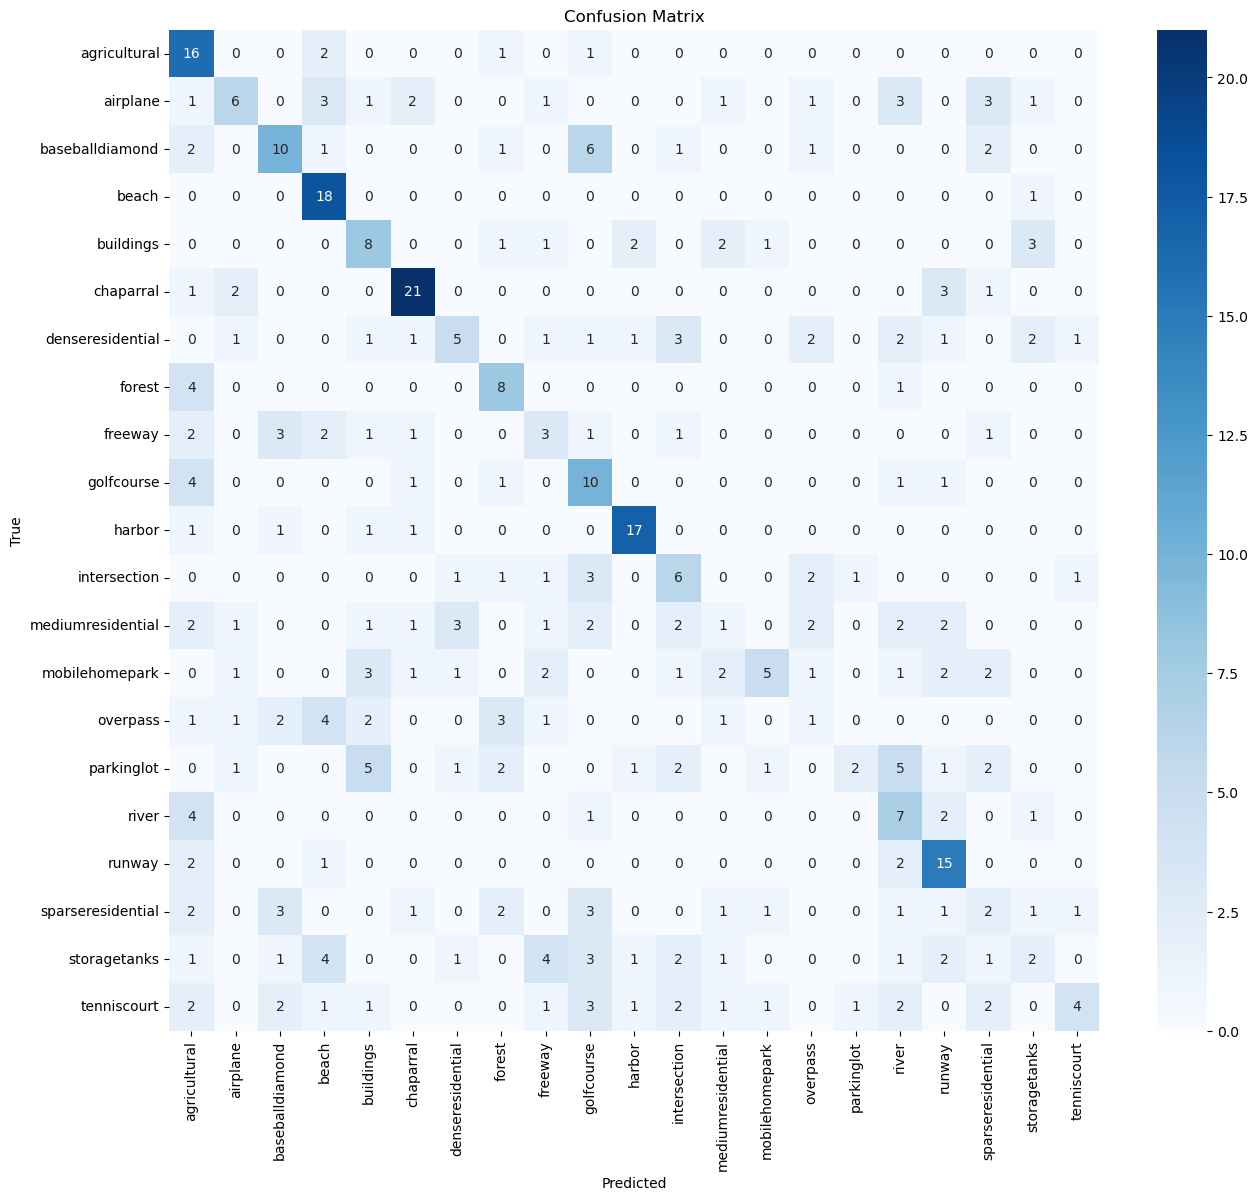
\includegraphics[width=6.85in]{pics/confusion_matrix.png}}
    \caption{Generated confusion matrix of the model [own figure]}
    \label{c_matrix}
\end{figure*}

%%%%%%%%%%%%%%%%%%%%%%%%%%%%%
% Discussion and conclusion %
%%%%%%%%%%%%%%%%%%%%%%%%%%%%%

\section{Discussion and conclusion}

The performance values of the model are comparably low, which is due to the fact that the model is not optimized and the data is not preprocessed.
Nevertheless, the model is able to classify some of the images correctly, which is clearly shown in the confusion matrix.
To optimize the model, the data could be selected more thoroughly for more distinguishable features and the model could be trained with more iterations or simply a larger dataset representing the important features of each class.

In the end, RandomForest seems to be a good choice for this classification task, because it is able to classify the images with a certain accuracy and provide a good starting point for further optimization.
In the process of writing the code for this project, it was also found that the \texttt{scikit-learn} package offers a lot of useful functions for data processing and model training, which makes it a good choice for tasks requiring machine learning algorithms.
Combining it with other packages like \texttt{seaborn} for visualization and \texttt{pandas} for data processing, it is possible to easily create a powerful tool for complex machine learning applications.

This paper shows that AI and specifically GeoAI provide useful tools for complex geographic analyses using machine learning algorithms and are valid research topics for the future.

%%%%%%%%%%%%%%%%
% Bibliography %
%%%%%%%%%%%%%%%%

\bibliographystyle{asmems4}
\bibliography{literature}

\end{document}
